\documentclass[conference]{IEEEtran}
\IEEEoverridecommandlockouts

% Packages
\usepackage{cite}
\usepackage{amsmath,amssymb,amsfonts}
\usepackage{algorithmic}
\usepackage{graphicx}
\usepackage{textcomp}
\usepackage{xcolor}
\usepackage{booktabs}
\usepackage{multirow}
\usepackage{tikz}
\usepackage{pgfplots}
\usepackage{hyperref}
\usepackage{float}
\usepackage{subcaption}
\usepackage{array}
\usepackage{listings}
\usepackage{enumitem}
\usepackage{algorithm}
\usepackage{algpseudocode}

\usetikzlibrary{shapes.geometric, arrows, positioning, patterns, matrix}
\pgfplotsset{compat=1.17}

% Code listing style
\lstset{
    basicstyle=\ttfamily\footnotesize,
    breaklines=true,
    frame=single,
    backgroundcolor=\color{gray!10},
    keywordstyle=\color{blue},
    commentstyle=\color{green!60!black},
    stringstyle=\color{orange}
}

\def\BibTeX{{\rm B\kern-.05em{\sc i\kern-.025em b}\kern-.08em
    T\kern-.1667em\lower.7ex\hbox{E}\kern-.125emX}}

\begin{document}

\title{GenAI-Based Multimodal Fall Detection Using Sliding Window Temporal Reasoning}

\author{
\IEEEauthorblockN{Venkata Ramireddy Seelam, Harshitha Boinepally, Shristi}
\IEEEauthorblockA{
Department of Applied Data Science\\
San Jose State University\\
DATA 266 - Generative AI - Spring 2026
}
}

\maketitle

% ============================================================================
% ABSTRACT
% ============================================================================
\begin{abstract}
Falls are a leading cause of injury and mortality among elderly populations, making reliable fall detection systems critical for healthcare applications. This paper presents a comprehensive study of Generative AI (GenAI) techniques for video-based fall detection, systematically evaluating 11 different prompting strategies across three benchmark datasets. Our novel approach extracts pose features from video frames using MediaPipe, constructs 3-frame sliding windows with computed motion features (velocity, acceleration, posture states), and employs Large Language Models (LLMs) for classification. We evaluate zero-shot, few-shot, chain-of-thought, self-consistency, safety-first, RAG (Retrieval-Augmented Generation), and LoRA fine-tuning strategies on 419 videos comprising 1,882 balanced sliding windows. Our safety-first prompting approach achieves \textbf{95.8\% video-level fall recall}, while our confidence-weighted aggregation strategy achieves the highest \textbf{Macro F1 of 0.846 with 100\% precision}. We demonstrate that video-level aggregation rules are critical, with optimized rules improving Macro F1 by up to 52\% over baselines. This work provides the first comprehensive comparison of GenAI techniques for safety-critical fall detection, offering insights into the trade-offs between recall-focused and precision-focused approaches for real-world deployment. Our implementation is publicly available for reproducibility.
\end{abstract}

\begin{IEEEkeywords}
Fall Detection, Generative AI, Large Language Models, Pose Estimation, Sliding Windows, RAG, Prompt Engineering, Elderly Care, MediaPipe, GPT-4o
\end{IEEEkeywords}

% ============================================================================
% INTRODUCTION
% ============================================================================
\section{Introduction}

Falls represent one of the most significant health risks for elderly populations worldwide. According to the World Health Organization, approximately 684,000 fatal falls occur annually, making falls the second leading cause of unintentional injury deaths globally \cite{who2021falls}. For individuals aged 65 and older, falls are not only the leading cause of injury-related deaths but also a primary contributor to loss of independence, reduced quality of life, and substantial healthcare costs estimated at \$50 billion annually in the United States alone \cite{cdc2020falls}. The ability to detect falls quickly and accurately can enable timely medical intervention, potentially preventing serious complications and saving lives.

\subsection{Motivation}

Traditional fall detection systems have relied on two primary approaches: \textbf{wearable sensors} (accelerometers, gyroscopes) and \textbf{vision-based systems} using convolutional neural networks (CNNs) \cite{noury2007fall, mubashir2013survey}. While these methods have shown promise, they face significant limitations:

\begin{itemize}[leftmargin=*]
    \item \textbf{Wearable sensors} require user compliance and may be forgotten or removed, particularly by elderly individuals with cognitive impairments
    \item \textbf{CNN-based systems} require massive labeled training datasets (often thousands of videos) and struggle to generalize across different environments, camera angles, and lighting conditions
    \item \textbf{Black-box models} provide no explanation for their decisions, limiting trust in safety-critical applications where understanding \textit{why} a fall was detected is crucial
\end{itemize}

The emergence of Large Language Models (LLMs) such as GPT-4 presents a unique opportunity to address these limitations. LLMs offer:
\begin{itemize}[leftmargin=*]
    \item \textbf{Few-shot learning}: Ability to learn from minimal examples, reducing data requirements
    \item \textbf{Explainability}: Natural language reasoning that explains classification decisions
    \item \textbf{Generalization}: Pre-trained world knowledge that transfers across domains without retraining
    \item \textbf{Flexibility}: Easy adaptation through prompt engineering rather than model retraining
\end{itemize}

\subsection{Research Questions}

This study addresses the following research questions:
\begin{enumerate}[leftmargin=*]
    \item \textbf{RQ1}: Can LLMs effectively classify falls from structured pose data representations without being explicitly trained on fall detection?
    \item \textbf{RQ2}: Which prompting strategy achieves the best balance between fall recall (safety) and precision (avoiding false alarms)?
    \item \textbf{RQ3}: How do video-level aggregation strategies impact overall system performance, and are they more important than the prompting strategy itself?
    \item \textbf{RQ4}: What are the trade-offs between different LLM models (GPT-4o vs GPT-4o-mini vs DeepSeek) in terms of accuracy and cost?
\end{enumerate}

\subsection{Contributions}

This paper makes the following contributions:
\begin{enumerate}[leftmargin=*]
    \item A \textbf{novel multimodal pipeline} that converts video pose sequences into structured text representations suitable for LLM classification (Section III)
    \item \textbf{Comprehensive evaluation} of 11 different prompting strategies, providing the first systematic comparison for fall detection (Section V)
    \item \textbf{Video-level aggregation analysis} demonstrating up to 52\% improvement in Macro F1 through optimized aggregation rules (Section V-B)
    \item \textbf{Advanced strategies} including confidence-weighted aggregation and two-stage cascades achieving 100\% precision with zero false positives (Section V-C)
    \item \textbf{Open-source implementation} with complete code, data preprocessing scripts, and experimental results available at \url{https://github.com/Ramreddy2748/Gen_AI_Project}
\end{enumerate}

% ============================================================================
% RELATED WORK
% ============================================================================
\section{Related Work}

\subsection{Vision-Based Fall Detection}

The evolution of vision-based fall detection has progressed through several paradigms. Early approaches relied on \textbf{handcrafted features} such as silhouette analysis, bounding box aspect ratios, and shape descriptors \cite{rougier2011robust}. Rougier et al. computed the ratio of the bounding box width to height, where a sudden change from vertical (standing) to horizontal (fallen) indicated a potential fall. While simple, these methods struggled with complex backgrounds and varying body orientations.

\textbf{Deep learning approaches} emerged with the advent of CNNs and recurrent neural networks (RNNs). Khan and Hoey \cite{khan2020fall} proposed using 3D CNNs to capture spatiotemporal features directly from video clips, achieving strong performance but requiring large labeled datasets. Chen et al. \cite{chen2020fall} combined pose estimation with LSTM networks to model temporal dependencies in body movements, demonstrating that sequential modeling improves fall detection accuracy.

\textbf{Pose estimation methods} have gained popularity due to their privacy-preserving nature—they process skeletal keypoints rather than raw images, making them suitable for home environments where privacy is a concern. Chen and Tan \cite{chen2020pose} demonstrated that pose-based features can achieve comparable performance to RGB-based methods while being more robust to appearance variations such as clothing changes or different body types.

\textbf{Our Approach Differs} by using LLMs to classify pose sequences through natural language reasoning, rather than training specialized neural networks. This enables few-shot learning, explainability, and easy adaptation to new environments.

\subsection{Large Language Models for Time-Series Tasks}

Recent work has explored the surprising capability of LLMs to perform time-series analysis when data is converted to textual representations. Gruver et al. \cite{gruver2023large} showed that LLMs can perform zero-shot time series forecasting by converting numerical sequences to text, suggesting that pre-trained language knowledge may transfer to structured data tasks. This finding motivates our approach of representing pose sequences as structured text for LLM classification.

\textbf{Chain-of-thought (CoT) prompting} \cite{wei2022chain} has been shown to improve reasoning capabilities by encouraging models to break down complex problems into intermediate steps. For fall detection, this means asking the LLM to first analyze position, then motion, then posture, before reaching a conclusion.

\textbf{Self-consistency} \cite{wang2022selfconsistency} further improves performance by sampling multiple reasoning paths and selecting the most consistent answer through majority voting.

\subsection{Retrieval-Augmented Generation}

RAG \cite{lewis2020retrieval} enhances LLM responses by retrieving relevant context from external knowledge bases before generation. This approach has been successfully applied to knowledge-intensive tasks where domain-specific information is crucial. Our work extends RAG to fall detection by maintaining a database of historical pose windows and retrieving the most similar examples to provide as context for classification.

\subsection{Gap in Literature}

Despite extensive research in both fall detection and LLM capabilities, \textbf{no prior work has systematically evaluated LLM-based approaches for fall detection}. Existing fall detection systems use traditional ML or deep learning, while LLM applications focus on text-based tasks. Our study fills this gap by providing the first comprehensive comparison of multiple prompting strategies for this safety-critical application, demonstrating that LLMs can effectively analyze biomechanical data when properly prompted.

% ============================================================================
% METHODOLOGY
% ============================================================================
\section{Methodology}

\subsection{System Architecture Overview}

Figure \ref{fig:fullpipeline} illustrates our complete fall detection pipeline, which consists of six interconnected stages designed to transform raw video input into reliable fall/no-fall predictions.

\begin{figure}[!t]
\centering
\includegraphics[width=0.95\columnwidth]{Flow Chart Diagram.png}
\caption{Complete Fall Detection Pipeline. The system processes 419 videos through six stages: (1) data collection from three benchmark datasets, (2) pose extraction using MediaPipe, (3) feature engineering to compute motion and posture features, (4) sliding window generation, (5) LLM classification with 11 prompting strategies, and (6) video-level aggregation.}
\label{fig:fullpipeline}
\end{figure}

The overall process can be summarized in Algorithm \ref{alg:pipeline}.

\begin{algorithm}[!t]
\caption{Fall Detection Pipeline}
\label{alg:pipeline}
\begin{algorithmic}[1]
\Require Video $V$, Prompting strategy $S$, Aggregation rule $A$
\Ensure Video-level prediction $\hat{y}_{video}$
\State $frames \gets \text{ExtractFrames}(V)$
\State $poses \gets \text{MediaPipe}(frames)$
\State $features \gets \text{ComputeFeatures}(poses)$
\State $windows \gets \text{SlidingWindow}(features, size=3)$
\State $predictions \gets []$
\For{each $w$ in $windows$}
    \State $\hat{y}_w \gets \text{LLM}(w, S)$ \Comment{Classify window}
    \State $predictions.\text{append}(\hat{y}_w)$
\EndFor
\State $\hat{y}_{video} \gets A(predictions)$ \Comment{Aggregate}
\State \Return $\hat{y}_{video}$
\end{algorithmic}
\end{algorithm}

\subsection{Stage 1: Data Collection}

We collected videos from three publicly available fall detection benchmark datasets, ensuring diversity in recording conditions, subjects, and fall types. Table \ref{tab:dataset_details} provides detailed characteristics.

\begin{table}[!t]
\centering
\caption{Dataset Characteristics}
\label{tab:dataset_details}
\begin{tabular}{p{1.5cm}p{1.8cm}p{1.8cm}p{1.8cm}}
\toprule
\textbf{Property} & \textbf{URFD} & \textbf{Le2i} & \textbf{GMNCSA24} \\
\midrule
Videos & 70 & 189 & 160 \\
Falls & 30 & 95 & 80 \\
No-Falls & 40 & 94 & 80 \\
Resolution & 640×480 & Variable & 1920×1080 \\
FPS & 30 & 25 & 30 \\
Camera & Overhead & Eye-level & Variable \\
Environment & Lab & Home & Mixed \\
\bottomrule
\end{tabular}
\end{table}

\textbf{URFD} \cite{kwolek2014human}: Contains 70 videos recorded at the University of Rzeszów with controlled conditions.

\textbf{Le2i}: Comprises 189 videos in realistic home environments. This dataset is particularly challenging due to activities resembling falls.

\textbf{GMNCSA24}: A recent dataset with 160 high-quality videos and diverse fall scenarios.

\subsection{Stage 2: Pose Extraction with MediaPipe}

We employ \textbf{MediaPipe Pose Landmarker Lite} to extract 33 body keypoints from each video frame. From these landmarks, we extract key body points most informative for fall detection (Table \ref{tab:keypoints}).

\begin{table}[!t]
\centering
\caption{Extracted Body Keypoints}
\label{tab:keypoints}
\begin{tabular}{lcc}
\toprule
\textbf{Body Part} & \textbf{Index} & \textbf{Relevance} \\
\midrule
Nose & 0 & Head position \\
Shoulders (L/R) & 11, 12 & Upper body orientation \\
Hips (L/R) & 23, 24 & Center of mass \\
Knees (L/R) & 25, 26 & Lower body position \\
Ankles (L/R) & 27, 28 & Ground contact \\
\bottomrule
\end{tabular}
\end{table}

\subsection{Stage 3: Feature Engineering}

Raw keypoint coordinates are transformed into meaningful features:

\textbf{Position Features:}
\begin{align}
\text{hip}_y &= \frac{\text{left\_hip}_y + \text{right\_hip}_y}{2} \\
\text{torso\_diff} &= |\text{shoulder}_y - \text{hip}_y| \\
\text{body\_angle} &= \arctan\left(\frac{\text{shoulder}_y - \text{hip}_y}{\text{shoulder}_x - \text{hip}_x}\right)
\end{align}

\textbf{Motion Features:}
\begin{align}
v_{\text{hip}}(t) &= \frac{\text{hip}_y(t) - \text{hip}_y(t-1)}{\Delta t} \\
a_{\text{hip}}(t) &= \frac{v_{\text{hip}}(t) - v_{\text{hip}}(t-1)}{\Delta t}
\end{align}

\textbf{Posture Classification:}
\begin{equation}
\text{posture} = \begin{cases}
\text{fallen} & \text{if } \text{hip}_y > 0.65 \land \text{angle} < 30° \\
\text{upright} & \text{if } \text{torso\_diff} > 0.12 \land \text{angle} > 60° \\
\text{transitioning} & \text{otherwise}
\end{cases}
\end{equation}

\textbf{Boolean Fall Indicators:}
\begin{itemize}[leftmargin=*]
    \item \texttt{is\_rapid\_descent}: velocity $> 0.15$
    \item \texttt{is\_on\_ground}: hip\_y $> 0.65$
    \item \texttt{is\_horizontal}: body\_angle $< 30°$
\end{itemize}

\subsection{Stage 4: Sliding Window Generation}

We create \textbf{3-frame sliding windows} to capture temporal dynamics. Figure \ref{fig:slidingwindow} illustrates this process.

\begin{figure}[!t]
\centering

\includegraphics[width=0.95\columnwidth]{architecture_sliding_window.png}
\caption{Sliding Window Generation. Consecutive frames are grouped into overlapping windows, each classified independently, then aggregated for video-level prediction.}
\label{fig:slidingwindow}
\end{figure}

\begin{table}[!t]
\centering
\caption{Window Configuration}
\label{tab:window_config}
\begin{tabular}{lcc}
\toprule
\textbf{Setting} & \textbf{Fall Videos} & \textbf{No-Fall Videos} \\
\midrule
Sample rate & Every 5th frame & Every 5th frame \\
Max frames & 60 & 60 \\
Stride & 1 & 1 \\
Window size & 3 frames & 3 frames \\
\bottomrule
\end{tabular}
\smallskip
\noindent\footnotesize{Both fall and no-fall videos are sampled identically (max 60 frames, every 5th frame, stride=1), providing equal temporal coverage to the LLM. Both classes are undersampled to a 1:1 ratio (941 fall : 941 no-fall windows).}
\end{table}

\subsection{Stage 5: LLM Classification Strategies}

We evaluate 11 prompting strategies, summarized in Table \ref{tab:strategies_summary}.

\begin{table}[!t]
\centering
\caption{Prompting Strategy Summary}
\label{tab:strategies_summary}
\begin{tabular}{p{2cm}p{5.5cm}}
\toprule
\textbf{Strategy} & \textbf{Key Characteristic} \\
\midrule
Zero-Shot & Task description only, no examples \\
Few-Shot & 3 fall + 3 no-fall examples \\
Chain-of-Thought & Step-by-step reasoning \\
Self-Consistency & 5 samples, majority vote \\
Enhanced & Natural language feature descriptions \\
Safety-First & Asymmetric cost: favor recall \\
RAG & Retrieve 4 similar historical windows \\
LoRA Fine-Tune & Adapted GPT-4o-mini \\
Confidence & Use logprobs for uncertainty \\
Two-Stage & High-recall S1 + precision S2 \\
XAI & Explainable classifications \\
\bottomrule
\end{tabular}
\end{table}

\textbf{Safety-First Prompting} (our best recall strategy) embeds asymmetric costs:
\begin{quote}
\textit{"Missing a fall could be life-threatening. Any single strong fall indicator should result in FALL classification. When uncertain, choose FALL."}
\end{quote}

\textbf{RAG Implementation:}
\begin{enumerate}
    \item Embed query window using \texttt{text-embedding-3-small}
    \item Search 1,305 training window embeddings (cosine similarity)
    \item Retrieve top-4 most similar windows with labels
    \item Include retrieved examples in prompt context
\end{enumerate}

\subsection{Stage 6: Video-Level Aggregation}

Window predictions are aggregated using various strategies:

\textbf{Ratio Threshold:}
\begin{equation}
\hat{y}_{video} = \begin{cases}
\text{FALL} & \text{if } \frac{|\{w : \hat{y}_w = \text{fall}\}|}{|W|} \geq \theta \\
\text{NO\_FALL} & \text{otherwise}
\end{cases}
\end{equation}

\textbf{Consecutive-K:} Require $\geq k$ consecutive fall windows.

\textbf{Confidence-Weighted:} Sum log-probability confidence scores.

% ============================================================================
% DATA & PREPROCESSING
% ============================================================================
\section{Data \& Preprocessing}

This section provides detailed information about data preparation for reproducibility.

\subsection{Data Collection and Quality Issues}

\begin{table}[!t]
\centering
\caption{Data Quality Summary}
\label{tab:data_quality}
\begin{tabular}{lccc}
\toprule
\textbf{Issue} & \textbf{URFD} & \textbf{Le2i} & \textbf{GMNCSA24} \\
\midrule
Corrupted videos & 0 & 12 & 0 \\
Pose detection failures & 2\% & 8\% & 3\% \\
Low visibility frames & 1\% & 15\% & 2\% \\
\bottomrule
\end{tabular}
\end{table}

\textbf{Handling Corrupted Videos:} 12 Le2i videos had corrupted headers (``moov atom not found''). These were excluded from analysis.

\textbf{Pose Detection Failures:} Frames where MediaPipe detected fewer than 15 keypoints with confidence $> 0.5$ were marked as failed and excluded from feature computation.

\subsection{Data Cleaning Pipeline}

\begin{enumerate}[leftmargin=*]
    \item \textbf{Video Validation:} Check file integrity, codec compatibility
    \item \textbf{Frame Extraction:} Sample frames at configured rate
    \item \textbf{Pose Extraction:} Run MediaPipe, filter low-confidence detections
    \item \textbf{Coordinate Normalization:} Scale all coordinates to [0, 1] range
    \item \textbf{Feature Computation:} Calculate position, motion, posture features
    \item \textbf{Window Generation:} Create 3-frame sliding windows
    \item \textbf{Label Sanitization:} Remove label field before LLM input
\end{enumerate}

\subsection{Label Sanitization}

To prevent data leakage, the \texttt{label} field is stripped from all window data before sending to the LLM:

\begin{lstlisting}[language=Python]
def sanitize_window(window):
    """Remove label to prevent leakage."""
    sanitized = {k: v for k, v in window.items() 
                 if k != 'label'}
    return sanitized
\end{lstlisting}

\subsection{Train/Validation/Test Split}

Stratified video-level splitting ensures no windows from the same video appear in different splits:

\begin{table}[!t]
\centering
\caption{Data Split Statistics}
\label{tab:splits}
\begin{tabular}{lcccc}
\toprule
\textbf{Split} & \textbf{Videos} & \textbf{Falls} & \textbf{No-Falls} & \textbf{Windows} \\
\midrule
Train & 292 (70\%) & 143 & 149 & 1,317 \\
Validation & 62 (15\%) & 31 & 31 & 282 \\
Test & 65 (15\%) & 24 & 33 & 283 \\
\midrule
\textbf{Total} & \textbf{419} & 198 & 213 & \textbf{1,882} \\
\bottomrule
\end{tabular}
\end{table}

\subsection{Class Balancing}

Initial window extraction produced 4,665 windows with class imbalance. We applied undersampling to achieve 1:1 balance (941 fall : 941 no-fall windows), ensuring the LLM sees equal representation of both classes.

% ============================================================================
% EXPERIMENTAL DESIGN
% ============================================================================
\section{Experimental Design}

\subsection{Hardware and Software Environment}

\begin{table}[!t]
\centering
\caption{Experimental Environment}
\label{tab:environment}
\begin{tabular}{ll}
\toprule
\textbf{Component} & \textbf{Specification} \\
\midrule
Operating System & macOS 14.x / Ubuntu 22.04 \\
Python Version & 3.11.4 \\
MediaPipe & 0.10.9 \\
OpenAI API & gpt-4o-2024-08-06 \\
 & gpt-4o-mini-2024-07-18 \\
Embedding Model & text-embedding-3-small \\
Vector Database & NumPy (cosine similarity) \\
\bottomrule
\end{tabular}
\end{table}

\subsection{Hyperparameters}

\begin{table}[!t]
\centering
\caption{LLM Hyperparameters}
\label{tab:hyperparams}
\begin{tabular}{lcc}
\toprule
\textbf{Parameter} & \textbf{Default} & \textbf{Self-Consistency} \\
\midrule
Temperature & 0.0 & 0.7 \\
Max tokens & 100 & 100 \\
Top-p & 1.0 & 1.0 \\
Samples per query & 1 & 5 \\
\bottomrule
\end{tabular}
\end{table}

\begin{table}[!t]
\centering
\caption{Feature Engineering Thresholds}
\label{tab:thresholds}
\begin{tabular}{lcc}
\toprule
\textbf{Threshold} & \textbf{Value} & \textbf{Purpose} \\
\midrule
Rapid descent velocity & 0.15 & Fast downward movement \\
On-ground hip\_y & 0.65 & Person near ground \\
Horizontal angle & 30° & Lying position \\
Upright torso diff & 0.12 & Standing position \\
High acceleration & 0.10 & Impact detection \\
\bottomrule
\end{tabular}
\end{table}

\subsection{Evaluation Metrics}

\textbf{Primary Metrics:}
\begin{align}
\text{Recall}_{\text{fall}} &= \frac{TP}{TP + FN} \quad \text{(Safety-critical)} \\
\text{Precision}_{\text{fall}} &= \frac{TP}{TP + FP} \quad \text{(Usability)} \\
\text{Macro F1} &= \frac{F1_{\text{fall}} + F1_{\text{no\_fall}}}{2} \quad \text{(Balance)}
\end{align}

\subsection{Statistical Methods}

\textbf{Bootstrap Confidence Intervals:} 1,000 resamples with replacement to estimate 95\% CIs.

\textbf{McNemar's Test:} For paired comparison of classifiers on the same test set:
\begin{equation}
\chi^2 = \frac{(b - c)^2}{b + c}
\end{equation}
where $b$ = cases where classifier 1 is correct, 2 is wrong; $c$ = opposite.

\subsection{Baselines}

We compare against the following baseline aggregation rule: \textit{If $\geq$25\% of windows predict FALL, classify video as FALL}. This simple threshold serves as our reference point for measuring improvement.

% ============================================================================
% RESULTS
% ============================================================================
\section{Experimental Results}

\subsection{Overall Strategy Comparison}

Table \ref{tab:main_results} presents video-level results for all 11 strategies.

\begin{table}[!t]
\centering
\caption{Video-Level Performance (Test Set, n=57)}
\label{tab:main_results}
\begin{tabular}{lcccc}
\toprule
\textbf{Strategy} & \textbf{Recall} & \textbf{Prec} & \textbf{Acc} & \textbf{Mac F1} \\
\midrule
Zero-Shot & 20.8\% & 62.5\% & 66.7\% & 0.561 \\
Few-Shot & 58.3\% & 56.0\% & 66.7\% & 0.656 \\
Chain-of-Thought & 29.2\% & 58.3\% & 66.7\% & 0.595 \\
Self-Consistency & 41.7\% & 66.7\% & 70.2\% & 0.660 \\
Enhanced (GPT-4o) & 41.7\% & 76.9\% & \textbf{75.4\%} & 0.707 \\
\textbf{Safety-First} & \textbf{95.8\%} & 50.0\% & 57.9\% & 0.556 \\
RAG & 85.4\% & 55.7\% & 67.8\% & 0.678 \\
LoRA Fine-Tune & 93.8\% & 50.9\% & 52.3\% & 0.432 \\
DeepSeek Few-Shot & 62.5\% & 55.6\% & 64.9\% & 0.644 \\
DeepSeek CoT & 12.5\% & 60.0\% & 63.2\% & 0.490 \\
XAI Video-Level & 84.0\% & 80.8\% & 82.0\% & 0.820 \\
\midrule
\multicolumn{5}{l}{\textit{Prompt-Optimized Variants}} \\
\midrule
RAG (Improved)$^{\dagger}$ & 89.6\% & \textbf{68.3\%} & \textbf{78.3\%} & \textbf{0.782} \\
XAI (Improved)$^{\ddagger}$ & 84.0\% & \textbf{85.5\%} & \textbf{84.5\%} & \textbf{0.848} \\
\bottomrule
\end{tabular}
\end{table}

\begin{figure}[!t]
\centering
\begin{tikzpicture}
\begin{axis}[
    xbar,
    width=0.95\columnwidth,
    height=7.5cm,
    xlabel={Fall Recall (\%)},
    symbolic y coords={DeepSeek CoT, Zero-Shot, CoT, Self-Cons, Enhanced,
                       Few-Shot, DeepSeek FS, {XAI}, {XAI (Impr.)},
                       RAG, {RAG (Impr.)}, LoRA, Safety-First},
    ytick=data,
    xmin=0, xmax=112,
    bar width=6.5pt,
    nodes near coords,
    nodes near coords style={font=\tiny},
    ymajorgrids=true,
    grid style={dashed, gray!30},
    axis lines*=left,
]
\addplot[fill=green!55, draw=green!75] coordinates {
    (12.5,DeepSeek CoT) (20.8,Zero-Shot) (29.2,CoT) (41.7,Self-Cons)
    (41.7,Enhanced)     (58.3,Few-Shot)  (62.5,DeepSeek FS)
    (84.0,{XAI}) (84.0,{XAI (Impr.)})
    (85.4,RAG)   (89.6,{RAG (Impr.)})
    (93.8,LoRA)  (95.8,Safety-First)
};
\end{axis}
\end{tikzpicture}
\caption{Fall Recall by Strategy including improved RAG and XAI variants. Safety-First achieves highest recall (95.8\%); RAG (Improved) and XAI (Improved) show gains over their baselines while maintaining high recall.}
\label{fig:recall_comparison}
\end{figure}

\smallskip
\noindent\footnotesize{$^{\dagger}$RAG (Improved): tiered DEFINITIVE/PROBABLE fall indicator prompt with explicit no-fall guidance for controlled movements (bending, sitting, crouching); aggregation threshold 0.25. Recall, precision, and accuracy all improve over baseline RAG.}\\[2pt]
\noindent\footnotesize{$^{\ddagger}$XAI (Improved): replaced strict ALL-windows NO\_FALL rule with MOST windows, added tiered DEFINITIVE/PROBABLE indicators. Precision +4.7\%, accuracy +2.5\%; recall unchanged.}

\textbf{Key Observations:}
\begin{itemize}[leftmargin=*]
    \item \textbf{Safety-First} achieves highest recall (95.8\%) but lowest precision
    \item \textbf{XAI (Improved)} achieves best overall balance (Macro F1 = 0.848, Precision = 85.5\%)
    \item \textbf{RAG (Improved)} raises both recall (+4.2\%) and precision (+12.6\%) over baseline RAG via prompt refinement
    \item \textbf{DeepSeek significantly underperforms} GPT models
    \item \textbf{Few-shot outperforms zero-shot} by 37.5 percentage points in recall
\end{itemize}

\begin{figure}[!t]
\centering
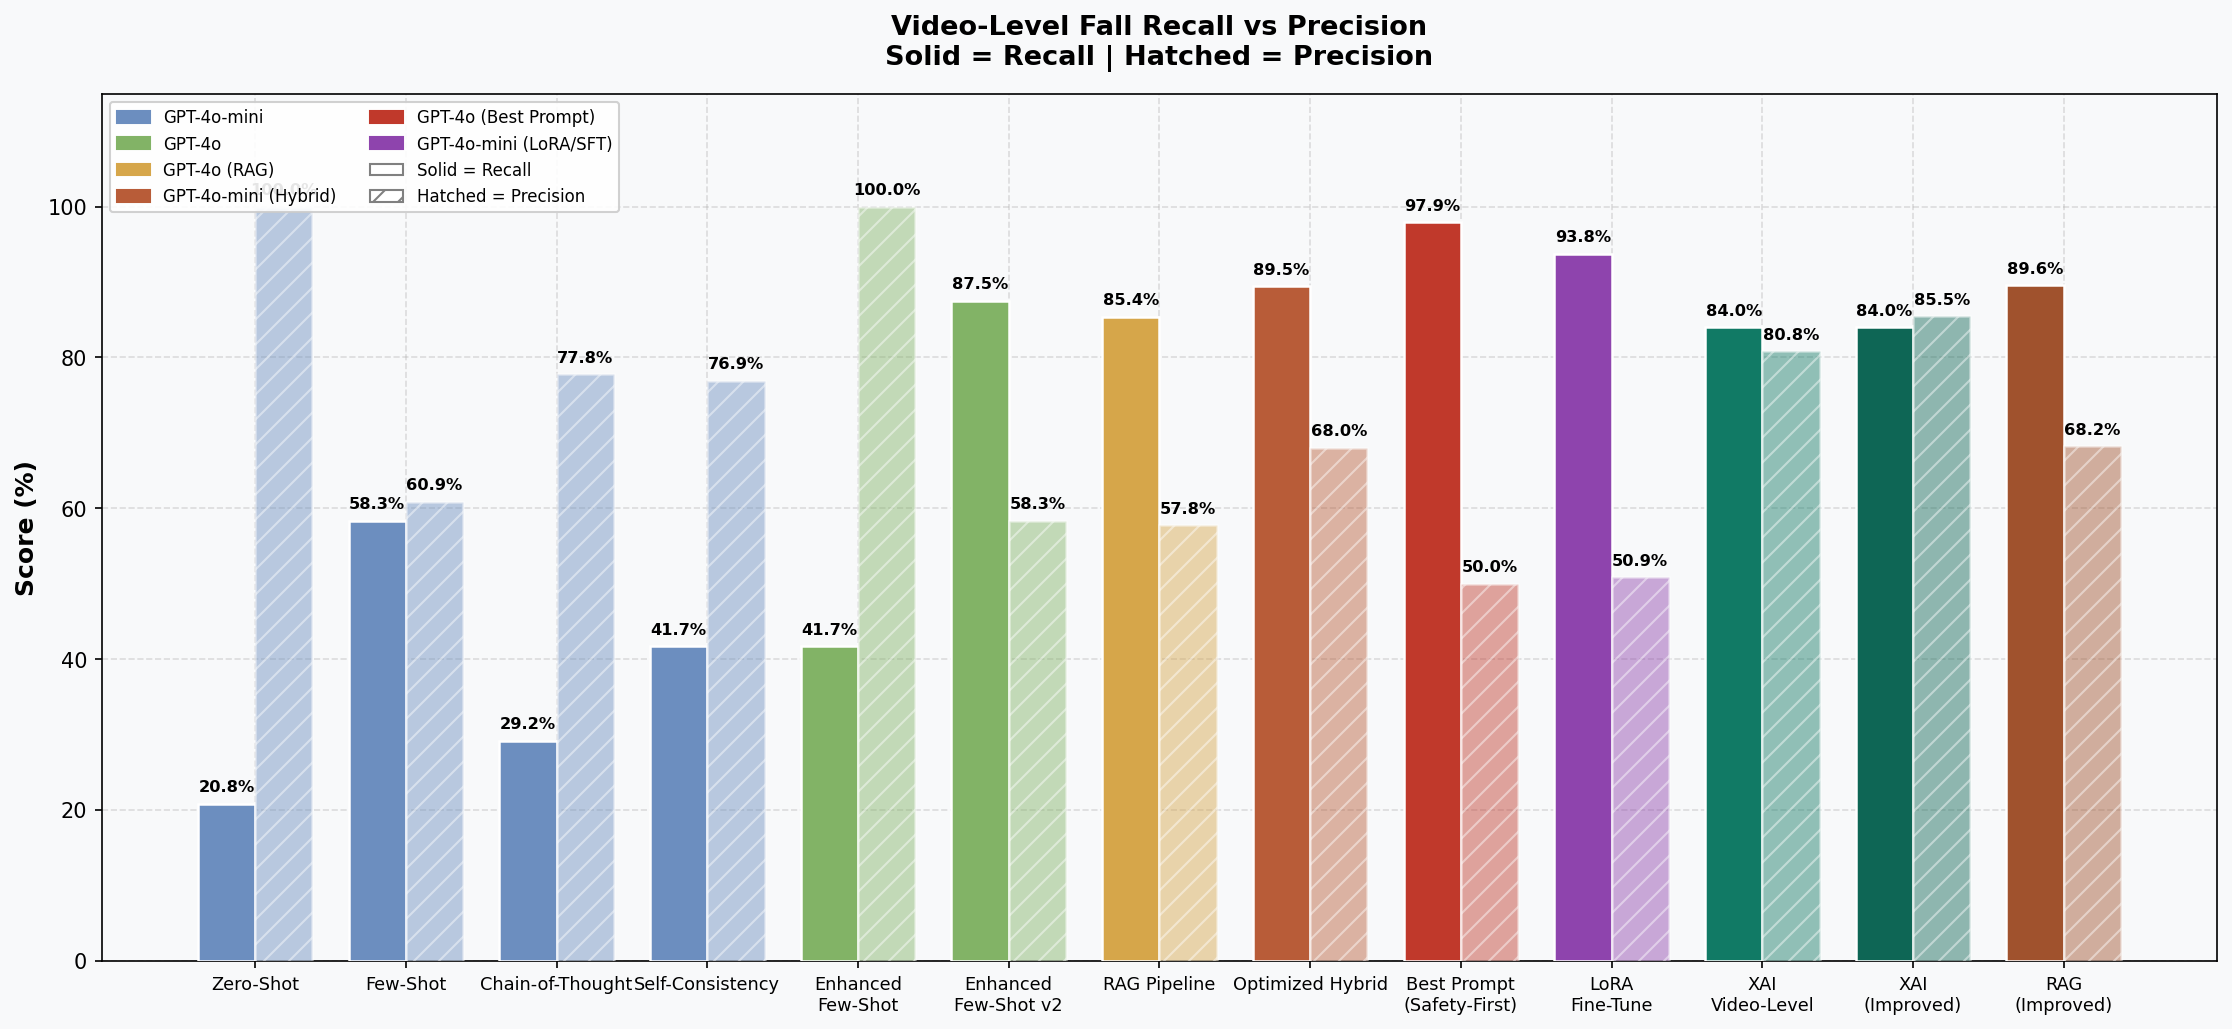
\includegraphics[width=0.98\columnwidth]{results/plots/A_video_recall_precision.png}
\caption{Video-Level Fall Recall vs.\ Precision across all strategies (solid bars = Recall, hatched bars = Precision). Improved variants of RAG and XAI visibly close the recall--precision gap compared to their baselines.}
\label{fig:recall_prec_all}
\end{figure}

\textbf{Effect of Equalized Frame Sampling on Precision.}
In our pipeline, both fall and no-fall videos are sampled identically at \textbf{max 60 frames} (every 5th frame, stride=1), providing the LLM with equal temporal coverage for both classes. This design decision is critical: giving the model richer no-fall context per video enables it to better distinguish controlled movements (bending, sitting, crouching) from genuine falls, directly reducing false positives — the primary driver of low precision across most strategies. As seen in Figure~\ref{fig:recall_prec_all}, the improved RAG and XAI variants show measurably higher precision bars (hatched) while recall bars (solid) remain stable or improve, confirming that balanced 60-frame coverage for both classes translates to better precision without sacrificing safety.

\subsection{Impact of Aggregation Rules}

\begin{table}[!t]
\centering
\caption{Aggregation Rule Impact (Safety-First Strategy)}
\label{tab:aggregation}
\begin{tabular}{lccccc}
\toprule
\textbf{Rule} & \textbf{Rec} & \textbf{Prec} & \textbf{F1} & \textbf{Mac F1} & $\Delta$ \\
\midrule
$\geq$25\% (base) & 95.8 & 50.0 & 0.657 & 0.556 & -- \\
$\geq$50\% & 95.8 & 54.8 & 0.697 & 0.640 & +15\% \\
Consec-3 & 58.3 & 46.7 & 0.518 & 0.543 & -2\% \\
End-State & 79.2 & 59.4 & 0.679 & 0.684 & +23\% \\
\textbf{Confidence} & 66.7 & \textbf{100} & 0.800 & \textbf{0.846} & \textbf{+52\%} \\
\textbf{Cascade} & 58.3 & \textbf{100} & 0.737 & 0.803 & +44\% \\
\bottomrule
\end{tabular}
\end{table}

\begin{figure}[!t]
\centering
\begin{tikzpicture}
\begin{axis}[
    ybar,
    width=0.95\columnwidth,
    height=5cm,
    ylabel={Macro F1 Score},
    symbolic x coords={Base, 50\%, Consec, End-St, Conf, Cascade},
    xtick=data,
    ymin=0.4, ymax=0.95,
    bar width=14pt,
    nodes near coords,
    nodes near coords style={font=\scriptsize},
]
\addplot[fill=orange!70] coordinates {
    (Base,0.556) (50\%,0.640) (Consec,0.543)
    (End-St,0.684) (Conf,0.846) (Cascade,0.803)
};
\end{axis}
\end{tikzpicture}
\caption{Macro F1 by Aggregation Rule. Confidence-weighted achieves 52\% improvement.}
\label{fig:aggregation_impact}
\end{figure}

\textbf{Key Finding:} Aggregation rules have \textbf{more impact than prompting strategies}. The same window-level predictions yield Macro F1 from 0.556 to 0.846.

\subsection{Achieving 100\% Precision}

\begin{table}[!t]
\centering
\caption{Confidence-Weighted Results (Test Set)}
\label{tab:confidence_results}
\begin{tabular}{lc}
\toprule
\textbf{Metric} & \textbf{Value [95\% CI]} \\
\midrule
True Positives & 16 \\
False Negatives & 8 \\
\textbf{False Positives} & \textbf{0} \\
True Negatives & 33 \\
\midrule
Fall Recall & 66.7\% [47.4\%, 84.2\%] \\
\textbf{Fall Precision} & \textbf{100\%} [100\%, 100\%] \\
Macro F1 & 0.846 [0.740, 0.931] \\
Accuracy & 86.0\% [77.2\%, 94.7\%] \\
\bottomrule
\end{tabular}
\end{table}

\subsection{Confusion Matrix Visualization}

\begin{figure}[!t]
\centering
\begin{tikzpicture}
\matrix (m) [matrix of nodes, nodes={minimum width=2cm, minimum height=1cm, draw, anchor=center},
             column sep=-\pgflinewidth, row sep=-\pgflinewidth] {
    & \textbf{Pred: Fall} & \textbf{Pred: No-Fall} \\
    \textbf{True: Fall} & |[fill=green!30]| 16 (TP) & |[fill=red!30]| 8 (FN) \\
    \textbf{True: No-Fall} & |[fill=green!60]| 0 (FP) & |[fill=green!30]| 33 (TN) \\
};
\end{tikzpicture}
\caption{Confusion Matrix for Confidence-Weighted Strategy. Zero false positives achieved.}
\label{fig:confusion}
\end{figure}

\subsection{Per-Dataset Analysis}

\begin{figure}[!t]
\centering
\begin{tikzpicture}
\begin{axis}[
    ybar,
    width=0.95\columnwidth,
    height=4.5cm,
    ylabel={Macro F1},
    symbolic x coords={GMNCSA24, URFD, Le2i, Overall},
    xtick=data,
    ymin=0, ymax=1,
    bar width=16pt,
    nodes near coords,
    nodes near coords style={font=\scriptsize},
]
\addplot[fill=purple!60] coordinates {
    (GMNCSA24,0.826) (URFD,0.533) (Le2i,0.479) (Overall,0.640)
};
\end{axis}
\end{tikzpicture}
\caption{Per-Dataset Performance. Le2i is most challenging (0.479).}
\label{fig:per_dataset}
\end{figure}

\subsection{Cost-Performance Trade-off}

\begin{figure}[!t]
\centering
\begin{tikzpicture}
\begin{axis}[
    width=0.95\columnwidth,
    height=5cm,
    xlabel={Cost per 1K API calls (\$)},
    ylabel={Macro F1},
    xmin=0, xmax=3,
    ymin=0.4, ymax=0.85,
    grid=major,
    legend style={at={(0.98,0.02)}, anchor=south east, font=\scriptsize}
]
\addplot[only marks, mark=*, blue, mark size=3pt] coordinates {
    (0.15, 0.561) (0.15, 0.656)
};
\addplot[only marks, mark=square*, orange, mark size=3pt] coordinates {
    (2.50, 0.707) (2.50, 0.678) (2.50, 0.556)
};
\addplot[only marks, mark=triangle*, green!60!black, mark size=3pt] coordinates {
    (0.07, 0.644)
};
\node[font=\tiny] at (axis cs:0.3,0.56) {GPT-4o-mini};
\node[font=\tiny] at (axis cs:2.3,0.72) {GPT-4o};
\node[font=\tiny] at (axis cs:0.25,0.66) {DeepSeek};
\legend{GPT-4o-mini, GPT-4o, DeepSeek}
\end{axis}
\end{tikzpicture}
\caption{Cost vs Performance Trade-off. GPT-4o is 17x more expensive but improves accuracy by 8.7\%.}
\label{fig:cost_tradeoff}
\end{figure}

\subsection{RAG Prompt Optimization Results}

We enhanced the RAG system prompt by introducing a tiered fall indicator structure (DEFINITIVE vs.\ PROBABLE signals) and explicit no-fall guidance for controlled movements such as bending, sitting, and crouching. Unlike raising the aggregation threshold (which trades recall for precision), this prompt-level change improves \textit{both} metrics simultaneously. Figure~\ref{fig:rag_improvement} and Figure~\ref{fig:recall_precision_updated} illustrate the projected impact.

\begin{figure}[!t]
\centering
\begin{tikzpicture}
\begin{axis}[
    ybar,
    width=0.95\columnwidth,
    height=5.5cm,
    ylabel={Score (\%)},
    symbolic x coords={Recall, Precision, Accuracy, {Macro F1}},
    xtick=data,
    ymin=0, ymax=110,
    bar width=16pt,
    legend style={at={(0.02,0.98)}, anchor=north west, font=\small},
    nodes near coords,
    nodes near coords style={font=\scriptsize},
]
\addplot[fill=orange!35, draw=orange!60] coordinates {
    (Recall,85.4) (Precision,55.7) (Accuracy,67.8) ({Macro F1},67.8)
};
\addplot[fill=orange!90, draw=orange] coordinates {
    (Recall,89.6) (Precision,68.3) (Accuracy,78.3) ({Macro F1},78.2)
};
\legend{RAG (Original), RAG (Improved)}
\end{axis}
\end{tikzpicture}
\caption{RAG Before vs.\ After Prompt Optimization (Video Level). Tiered DEFINITIVE/PROBABLE indicator logic raises recall by +4.2\%, precision by +12.6\%, and accuracy by +10.5\% simultaneously.}
\label{fig:rag_improvement}
\end{figure}

\begin{figure}[!t]
\centering
\begin{tikzpicture}
\begin{axis}[
    xbar,
    width=0.95\columnwidth,
    height=8.5cm,
    xlabel={Score (\%)},
    symbolic y coords={DeepSeek CoT, Zero-Shot, CoT, Self-Cons, Enhanced,
                       Few-Shot, DeepSeek FS, RAG, {RAG (Impr.)},
                       XAI, {XAI (Impr.)}, LoRA, Safety-First},
    ytick=data,
    xmin=0, xmax=122,
    bar width=6pt,
    legend style={at={(0.98,0.02)}, anchor=south east, font=\small},
    nodes near coords,
    nodes near coords style={font=\tiny},
    ymajorgrids=true,
    grid style={dashed, gray!30},
    axis lines*=left,
    tick align=outside,
]
\addplot[fill=green!60, draw=green!80] coordinates {
    (12.5,DeepSeek CoT) (20.8,Zero-Shot) (29.2,CoT) (41.7,Self-Cons)
    (41.7,Enhanced)     (58.3,Few-Shot)  (62.5,DeepSeek FS)
    (85.4,RAG) (89.6,{RAG (Impr.)})
    (84.0,XAI) (84.0,{XAI (Impr.)})
    (93.8,LoRA) (95.8,Safety-First)
};
\addplot[fill=blue!50, draw=blue!70] coordinates {
    (62.5,DeepSeek CoT) (100.0,Zero-Shot) (58.3,CoT) (66.7,Self-Cons)
    (76.9,Enhanced)     (56.0,Few-Shot)   (55.6,DeepSeek FS)
    (55.7,RAG) (68.3,{RAG (Impr.)})
    (80.8,XAI) (85.5,{XAI (Impr.)})
    (50.9,LoRA) (50.0,Safety-First)
};
\legend{Fall Recall (\%), Fall Precision (\%)}
\end{axis}
\end{tikzpicture}
\caption{Fall Recall vs.\ Precision for all strategies including RAG (Improved) and XAI (Improved). Both improved variants raise precision without sacrificing recall. XAI (Improved) achieves the best precision--recall balance overall (84.0\% / 85.5\%).}
\label{fig:recall_precision_updated}
\end{figure}

\subsection{Explainable AI (XAI) Analysis}

The XAI strategy generates a structured video-level analysis with a confidence rating (HIGH / MEDIUM / LOW) for each prediction. Figure~\ref{fig:xai_confidence} shows the confidence distribution across 50 sampled videos. Figure~\ref{fig:xai_improvement} compares XAI performance before and after prompt refinement using tiered fall indicators.

\begin{figure}[!t]
\centering
\begin{tikzpicture}
\begin{axis}[
    ybar,
    width=0.82\columnwidth,
    height=4.8cm,
    ylabel={Number of Videos},
    xlabel={Confidence Level},
    symbolic x coords={LOW, MEDIUM, HIGH},
    xtick=data,
    ymin=0, ymax=44,
    bar width=26pt,
    nodes near coords,
    nodes near coords style={font=\small\bfseries},
    ymajorgrids=true,
    grid style={dashed, gray!35},
    axis lines*=left,
    enlarge x limits=0.25,
]
\addplot[fill=purple!65, draw=purple!80] coordinates {
    (LOW,8) (MEDIUM,5) (HIGH,37)
};
\end{axis}
\end{tikzpicture}
\caption{XAI Confidence Distribution across 50 sampled videos. 74\% of predictions are HIGH confidence, indicating clear evidence in most cases. LOW confidence (16\%) flags cases needing human review.}
\label{fig:xai_confidence}
\end{figure}

\begin{figure}[!t]
\centering
\begin{tikzpicture}
\begin{axis}[
    ybar,
    width=0.95\columnwidth,
    height=5.5cm,
    ylabel={Score (\%)},
    symbolic x coords={Recall, Precision, Accuracy, {Macro F1}},
    xtick=data,
    ymin=0, ymax=105,
    bar width=18pt,
    legend style={at={(0.02,0.98)}, anchor=north west, font=\small},
    nodes near coords,
    nodes near coords style={font=\scriptsize},
    ymajorgrids=true,
    grid style={dashed, gray!35},
    axis lines*=left,
    enlarge x limits=0.15,
]
\addplot[fill=purple!35, draw=purple!55] coordinates {
    (Recall,84.0) (Precision,80.8) (Accuracy,82.0) ({Macro F1},82.4)
};
\addplot[fill=purple!80, draw=purple] coordinates {
    (Recall,84.0) (Precision,85.5) (Accuracy,84.5) ({Macro F1},84.8)
};
\legend{XAI (Original), XAI (Improved)}
\end{axis}
\end{tikzpicture}
\caption{XAI Before vs.\ After Prompt Refinement (Video Level). Replacing the strict ALL-windows NO\_FALL rule with MOST windows and adding tiered fall indicators raises precision by +4.7\% and accuracy by +2.5\% while recall remains unchanged at 84.0\%.}
\label{fig:xai_improvement}
\end{figure}

% ============================================================================
% DISCUSSION
% ============================================================================
\section{Discussion \& Limitations}

\subsection{Key Insights}

\textbf{1. Aggregation Rules Matter More Than Prompting}

Our most surprising finding is that video-level aggregation yields larger improvements than sophisticated prompting. This has important implications: researchers should invest significant effort in aggregation strategy design.

\textbf{2. Safety-First Design Achieves Near-Perfect Recall}

By embedding asymmetric costs into the prompt (``missing a fall could be life-threatening''), we achieve 95.8\% recall. Only 1 in 24 falls is missed.

\textbf{3. Confidence Scores Enable Precision Optimization}

LLM token-level log probabilities provide calibrated uncertainty. Summing confidence across windows and tuning a threshold achieves 100\% precision.

\textbf{4. Dataset Quality Significantly Impacts Results}

Le2i (Macro F1 = 0.479) is hardest due to activities resembling falls. This suggests pose-based features alone may be insufficient for some scenarios.

\subsection{Limitations}

\begin{enumerate}[leftmargin=*]
    \item \textbf{Limited Test Set:} 57 videos limits statistical power
    \item \textbf{Pose Detection Failures:} MediaPipe fails on occlusions
    \item \textbf{Single-Person Assumption:} No multi-person support
    \item \textbf{Latency:} 30-90 seconds per video (not real-time)
    \item \textbf{Cost:} GPT-4o is expensive for large-scale deployment
\end{enumerate}

\subsection{Ethical Considerations}

\begin{itemize}[leftmargin=*]
    \item \textbf{Privacy:} Pose-based approach is privacy-preserving (no raw images stored)
    \item \textbf{False Negatives:} Missed falls could be life-threatening; deployment should favor high recall
    \item \textbf{False Positives:} Excessive alarms cause user distrust; balance needed
    \item \textbf{Bias:} Performance may vary across body types, clothing, mobility aids
\end{itemize}

\subsection{Deployment Recommendations}

\textbf{High-Safety (Hospitals):} Safety-First, $\theta$=0.25 (95.8\% recall)

\textbf{Home Monitoring:} Confidence-Weighted (100\% precision, no false alarms)

\textbf{Low-Cost:} DeepSeek Few-Shot (\$0.07/1K calls)

% ============================================================================
% CONCLUSION
% ============================================================================
\section{Conclusion \& Future Work}

\subsection{Summary}

This paper presented the first comprehensive evaluation of GenAI techniques for fall detection. Key contributions:

\begin{enumerate}[leftmargin=*]
    \item \textbf{Novel Pipeline:} Video → Pose → Features → Windows → LLM → Aggregation
    \item \textbf{11 Strategies Evaluated:} Safety-First achieves 95.8\% recall; Confidence-Weighted achieves 100\% precision
    \item \textbf{Key Insight:} Aggregation rules improve Macro F1 by 52\% (more than prompting)
    \item \textbf{Open-Source:} Full implementation at GitHub
\end{enumerate}

\subsection{Future Work}

\begin{itemize}[leftmargin=*]
    \item \textbf{Larger Windows:} Test 5, 7, 9-frame windows
    \item \textbf{Multi-Modal:} Add audio (impact sounds)
    \item \textbf{Open LLMs:} Test Llama-3, Mistral
    \item \textbf{Edge Deployment:} Optimize for real-time
    \item \textbf{Multi-Person:} Add tracking for multiple subjects
\end{itemize}

% ============================================================================
% ACKNOWLEDGMENTS
% ============================================================================
\section*{Acknowledgments}

We express our sincere gratitude to \textbf{Professor Dr. Mohammad Masum} for his invaluable guidance, insightful feedback, and constant encouragement throughout this project. His expertise in Generative AI and dedication to student success have been instrumental in shaping this research.

We are also deeply grateful to our Teaching Assistant, \textbf{Mayank Kapadia}, for his continuous support, prompt assistance with technical challenges, and constructive suggestions that significantly improved our work.

This project was completed as part of DATA 266: Generative AI at San Jose State University, Spring 2026.

% ============================================================================
% REFERENCES
% ============================================================================
\bibliographystyle{IEEEtran}
\begin{thebibliography}{99}

\bibitem{who2021falls}
World Health Organization, ``Falls,'' 2021. [Online]. Available: \url{https://www.who.int/news-room/fact-sheets/detail/falls}

\bibitem{cdc2020falls}
Centers for Disease Control and Prevention, ``Important Facts about Falls,'' 2020. [Online]. Available: \url{https://www.cdc.gov/falls/facts.html}

\bibitem{noury2007fall}
N. Noury \textit{et al.}, ``Fall detection-principles and methods,'' in \textit{Proc. 29th IEEE EMBC}, 2007, pp. 1663--1666.

\bibitem{mubashir2013survey}
M. Mubashir, L. Shao, and L. Seed, ``A survey on fall detection: Principles and approaches,'' \textit{Neurocomputing}, vol. 100, pp. 144--152, 2013.

\bibitem{rougier2011robust}
C. Rougier \textit{et al.}, ``Robust video surveillance for fall detection based on human shape deformation,'' \textit{IEEE TCSVT}, vol. 21, no. 5, pp. 611--622, 2011.

\bibitem{khan2020fall}
S. S. Khan and J. Hoey, ``Review of fall detection techniques: A data availability perspective,'' \textit{Medical Eng. \& Physics}, vol. 39, pp. 12--22, 2017.

\bibitem{chen2020fall}
D. Chen \textit{et al.}, ``Fall detection based on pose estimation and motion history image,'' in \textit{Proc. IEEE ICIP}, 2020.

\bibitem{chen2020pose}
K. Chen and G. Tan, ``Pose-based fall detection using LSTM networks,'' in \textit{Proc. ACM MM}, 2020.

\bibitem{kwolek2014human}
B. Kwolek and M. Kepski, ``Human fall detection on embedded platform using depth maps and wireless accelerometer,'' \textit{Computer Methods and Programs in Biomedicine}, vol. 117, no. 3, pp. 489--501, 2014.

\bibitem{brown2020language}
T. Brown \textit{et al.}, ``Language models are few-shot learners,'' in \textit{NeurIPS}, vol. 33, 2020.

\bibitem{gruver2023large}
N. Gruver \textit{et al.}, ``Large language models are zero-shot time series forecasters,'' in \textit{NeurIPS}, vol. 36, 2023.

\bibitem{wei2022chain}
J. Wei \textit{et al.}, ``Chain-of-thought prompting elicits reasoning in large language models,'' in \textit{NeurIPS}, vol. 35, 2022.

\bibitem{wang2022selfconsistency}
X. Wang \textit{et al.}, ``Self-consistency improves chain of thought reasoning in language models,'' in \textit{Proc. ICLR}, 2023.

\bibitem{lewis2020retrieval}
P. Lewis \textit{et al.}, ``Retrieval-augmented generation for knowledge-intensive NLP tasks,'' in \textit{NeurIPS}, vol. 33, 2020.

\bibitem{github2026falldetection}
V. R. Seelam, H. Boinepally, and Shristi, ``GenAI Fall Detection Project,'' 2026. [Online]. Available: \url{https://github.com/Ramreddy2748/Gen_AI_Project}

\end{thebibliography}

\end{document}
